\documentclass[tikz,dvipsnames]{standalone}
\usetikzlibrary{backgrounds}
\usetikzlibrary{calc}
\usetikzlibrary{arrows.meta}
\usetikzlibrary{positioning} 
\usepackage{amsmath}

\begin{document}
 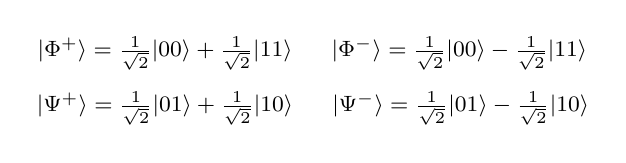
\begin{tikzpicture}[
    show background rectangle,
    tight background=0,
    font=\footnotesize,
    background rectangle/.style={fill=white},
%     node distance=0.10cm and 2cm,
 ]
    \node (X0) {$|\Phi^+ \rangle= \tfrac{1}{\sqrt{2}}|00\rangle+\tfrac{1}{\sqrt{2}}|11\rangle$};
    \node[right=0.25cm of X0] (X1) {$|\Phi^- \rangle= \tfrac{1}{\sqrt{2}}|00\rangle-\tfrac{1}{\sqrt{2}}|11\rangle $};
    \node[below=0.03cm of X0] (X2) {$ |\Psi^+ \rangle= \tfrac{1}{\sqrt{2}}|01\rangle+\tfrac{1}{\sqrt{2}}|10\rangle$};
    \node[right=0.25cm of X2] (X3) {$|\Psi^- \rangle= \tfrac{1}{\sqrt{2}}|01\rangle-\tfrac{1}{\sqrt{2}}|10\rangle $};
    
\end{tikzpicture}
\end{document}
